% !TeX program = xelatex
\documentclass{article}
\usepackage{kotex}
\usepackage[a4paper,left=3cm, right=3cm, top=2cm, bottom=2cm]{geometry}
\usepackage{amsmath}
\usepackage{graphicx}
\usepackage{caption}
\usepackage{setspace}
\usepackage{xcolor}
\usepackage{titlesec}
\usepackage{amssymb}
\usepackage{tcolorbox}
\usepackage{amsthm}
\usepackage{multirow}
\usepackage{array}
\usepackage{tikz}
\usetikzlibrary{positioning,arrows.meta,calc,matrix}
\usepackage{pgfplots}
\pgfplotsset{compat=1.18}

\title{7.2 Orthogonal Diagonalization}
\date{}
\author{}
\setstretch{1.3}

\titleformat{name=\section, numberless}
  {\normalfont\large\bfseries\color{blue}}{}
  {0pt}{}
\geometry{a4paper, margin=1in}

\newcommand{\redheading}[1]{{\vspace{2mm}\noindent\Large\bfseries\color{red!55!black} #1\par}\vspace{2mm}}

\newtheoremstyle{mystyle}
  {}{}{\itshape}{}{\bfseries}{.}{.5em}{}
\theoremstyle{mystyle}

\begin{document}
\maketitle

{\itshape\color{blue!45!black}
In this section we will be concerned with the problem of diagonalizing a symmetric
matrix $A$. As we will see, this problem is closely related to finding an orthonormal
basis for $\mathbb{R}^n$ that consists of eigenvectors of $A$. Problems of this type
are important because many of the matrices that arise in applications are symmetric.\par}

\vspace{2mm}

\redheading{The Orthogonal Diagonalization Problem}

Recall from Section 5.2 that two square matrices $A$ and $B$ are \emph{similar} if there
is an invertible matrix $P$ such that $P^{-1}AP = B$. Here we focus on the special case
where $P$ is orthogonal.

\begin{tcolorbox}[colback=teal!4, colframe=teal!65!black,
  title={\textbf{Definition 1}}, boxrule=0.5mm, arc=3mm]
Square matrices $A$ and $B$ are \textbf{orthogonally similar} if there is an orthogonal
matrix $P$ such that $B = P^T AP$. If $A$ is orthogonally similar to a diagonal matrix
$D$, we say $A$ is \textbf{orthogonally diagonalizable} and that $P$
\textbf{orthogonally diagonalizes} $A$.
\end{tcolorbox}

If $P^T AP = D$, multiplying left by $P$ and right by $P^T$ and using $PP^T = I$ yields
\begin{equation}
  A = PDP^T \tag{2}
\end{equation}
Transposing both sides and noting a diagonal matrix satisfies $D^T = D$:
\[
  A^T = (PDP^T)^T = (P^T)^T D^T P^T = PDP^T = A
\]
so $A$ must be symmetric. This proves one direction of the following theorem.

\redheading{Conditions for Orthogonal Diagonalizability}

\begin{tcolorbox}[colback=red!4, colframe=red!60!black,
  title={\textbf{Theorem 7.2.1}}, boxrule=0.5mm, arc=3mm]
If $A$ is an $n\times n$ matrix with real entries, the following are equivalent:
\begin{enumerate}
  \item[(a)] $A$ is orthogonally diagonalizable.
  \item[(b)] $A$ has an orthonormal set of $n$ eigenvectors.
  \item[(c)] $A$ is symmetric.
\end{enumerate}
\end{tcolorbox}

\textit{Proof.}

\textbf{$(a)\Rightarrow(b)$} If $A$ is orthogonally diagonalizable, there is an orthogonal
$P$ with $P^{-1}AP$ diagonal. As shown in Formula (2) in the proof of Theorem 5.2.1, the
$n$ column vectors of $P$ are eigenvectors of $A$. Since $P$ is orthogonal, those columns
are orthonormal, so $A$ has $n$ orthonormal eigenvectors.

\textbf{$(b)\Rightarrow(a)$} Suppose $A$ has an orthonormal set of $n$ eigenvectors
$\{\mathbf{p}_1,\ldots,\mathbf{p}_n\}$. The matrix $P$ with these as columns diagonalizes
$A$ (Theorem 5.2.1). Since the eigenvectors are orthonormal, $P$ is orthogonal, so $P$
orthogonally diagonalizes $A$.

\textbf{$(a)\Rightarrow(c)$} Shown above: $P^T AP = D$ implies $A = PDP^T$, which gives
$A^T = PD^TP^T = PDP^T = A$.

\textbf{$(c)\Rightarrow(a)$} The proof that every real symmetric matrix is orthogonally
diagonalizable is beyond the scope of this text; the structure of the argument is outlined
in Exercise~31. $\blacksquare$

\redheading{Properties of Symmetric Matrices}

To devise an algorithm for orthogonally diagonalizing a symmetric matrix, we need the
following critical properties.

\begin{tcolorbox}[colback=red!4, colframe=red!60!black,
  title={\textbf{Theorem 7.2.2}}, boxrule=0.5mm, arc=3mm]
If $A$ is a symmetric matrix with real entries, then:
\begin{enumerate}
  \item[(a)] The eigenvalues of $A$ are all real numbers.
  \item[(b)] Eigenvectors from different eigenspaces are orthogonal.
\end{enumerate}
\end{tcolorbox}

Part~(a) requires results about complex vector spaces and is discussed in Section~7.5.

\textit{Proof of (b).} Let $\mathbf{v}_1$ and $\mathbf{v}_2$ be eigenvectors of $A$
for distinct eigenvalues $\lambda_1$ and $\lambda_2$. Using Formula~(26) of Section~3.2
and the symmetry $A = A^T$:
\begin{equation}
  A\mathbf{v}_1\cdot\mathbf{v}_2
  = \mathbf{v}_1\cdot A^T\mathbf{v}_2
  = \mathbf{v}_1\cdot A\mathbf{v}_2 \tag{3}
\end{equation}
Since $A\mathbf{v}_i = \lambda_i\mathbf{v}_i$, equation (3) gives
$\lambda_1\mathbf{v}_1\cdot\mathbf{v}_2 = \mathbf{v}_1\cdot\lambda_2\mathbf{v}_2$, i.e.,
\begin{equation}
  (\lambda_1 - \lambda_2)(\mathbf{v}_1\cdot\mathbf{v}_2) = 0 \tag{4}
\end{equation}
Since $\lambda_1\neq\lambda_2$, we conclude $\mathbf{v}_1\cdot\mathbf{v}_2 = 0$. $\blacksquare$

Theorem~7.2.2 yields the following procedure. Its correctness follows because eigenvectors
from \emph{different} eigenspaces are already orthogonal (by Theorem~7.2.2(b)), and
Gram--Schmidt makes eigenvectors within the \emph{same} eigenspace orthonormal.

\begin{tcolorbox}[colback=teal!4, colframe=teal!65!black,
  title={Orthogonally Diagonalizing an $n\times n$ Symmetric Matrix},
  fonttitle=\bfseries, boxrule=0.5mm, arc=3mm]
\textbf{\color{teal!70!black}Step 1.} Find a basis for each eigenspace of $A$.

\textbf{\color{teal!70!black}Step 2.} Apply the Gram--Schmidt process to each of those
bases to obtain an orthonormal basis for each eigenspace.

\textbf{\color{teal!70!black}Step 3.} Form the matrix $P$ whose columns are the vectors
constructed in Step~2. This matrix orthogonally diagonalizes $A$, and the diagonal of
$D = P^T AP$ lists the eigenvalues in the same order as their corresponding eigenvectors
in $P$.
\end{tcolorbox}

\subsection*{EXAMPLE 1 | Orthogonally Diagonalizing a Symmetric Matrix}

Find an orthogonal matrix $P$ that diagonalizes
\[
  A = \begin{bmatrix}4&2&2\\2&4&2\\2&2&4\end{bmatrix}
\]

\textbf{SOLUTION:} The characteristic equation is
\[
  \det(\lambda I - A) = \det\begin{bmatrix}\lambda-4&-2&-2\\-2&\lambda-4&-2\\-2&-2&\lambda-4\end{bmatrix}
  = (\lambda-2)^2(\lambda-8) = 0
\]
so the distinct eigenvalues are $\lambda=2$ (mult.~2) and $\lambda=8$ (mult.~1).

\textbf{Eigenspace for $\lambda=2$:} Solving $(2I-A)\mathbf{x}=\mathbf{0}$ gives basis
\begin{equation}
  \mathbf{u}_1 = \begin{bmatrix}-1\\1\\0\end{bmatrix}, \qquad
  \mathbf{u}_2 = \begin{bmatrix}-1\\0\\1\end{bmatrix} \tag{5}
\end{equation}
Applying Gram--Schmidt to $\{\mathbf{u}_1,\mathbf{u}_2\}$ yields orthonormal eigenvectors (verify):
\begin{equation}
  \mathbf{v}_1 = \begin{bmatrix}-\tfrac{1}{\sqrt{2}}\\[3pt]\tfrac{1}{\sqrt{2}}\\[3pt]0\end{bmatrix},
  \qquad
  \mathbf{v}_2 = \begin{bmatrix}-\tfrac{1}{\sqrt{6}}\\[3pt]-\tfrac{1}{\sqrt{6}}\\[3pt]\tfrac{2}{\sqrt{6}}\end{bmatrix}
  \tag{6}
\end{equation}

\textbf{Eigenspace for $\lambda=8$:} Solving $(8I-A)\mathbf{x}=\mathbf{0}$ gives basis
$\mathbf{u}_3=[1,1,1]^T$. Normalizing:
\[
  \mathbf{v}_3 = \begin{bmatrix}\tfrac{1}{\sqrt{3}}\\[3pt]\tfrac{1}{\sqrt{3}}\\[3pt]\tfrac{1}{\sqrt{3}}\end{bmatrix}
\]

Using $\mathbf{v}_1, \mathbf{v}_2, \mathbf{v}_3$ as column vectors:
\[
  P = \begin{bmatrix}
        -\tfrac{1}{\sqrt{2}} & -\tfrac{1}{\sqrt{6}} & \tfrac{1}{\sqrt{3}}\\[4pt]
        \tfrac{1}{\sqrt{2}}  & -\tfrac{1}{\sqrt{6}} & \tfrac{1}{\sqrt{3}}\\[4pt]
        0                   & \tfrac{2}{\sqrt{6}}  & \tfrac{1}{\sqrt{3}}
      \end{bmatrix}
\]
which orthogonally diagonalizes $A$. One can verify (verify):
\[
  P^T AP =
  \begin{bmatrix}-\tfrac{1}{\sqrt{2}}&\tfrac{1}{\sqrt{2}}&0\\[3pt]
                 -\tfrac{1}{\sqrt{6}}&-\tfrac{1}{\sqrt{6}}&\tfrac{2}{\sqrt{6}}\\[3pt]
                 \tfrac{1}{\sqrt{3}}&\tfrac{1}{\sqrt{3}}&\tfrac{1}{\sqrt{3}}\end{bmatrix}
  \begin{bmatrix}4&2&2\\2&4&2\\2&2&4\end{bmatrix}
  \begin{bmatrix}-\tfrac{1}{\sqrt{2}}&-\tfrac{1}{\sqrt{6}}&\tfrac{1}{\sqrt{3}}\\[3pt]
                 \tfrac{1}{\sqrt{2}}&-\tfrac{1}{\sqrt{6}}&\tfrac{1}{\sqrt{3}}\\[3pt]
                 0&\tfrac{2}{\sqrt{6}}&\tfrac{1}{\sqrt{3}}\end{bmatrix}
  = \begin{bmatrix}2&0&0\\0&2&0\\0&0&8\end{bmatrix}
\]

\redheading{Spectral Decomposition}

If $A$ is a symmetric matrix orthogonally diagonalized by
$P = [\mathbf{u}_1\ \mathbf{u}_2\ \cdots\ \mathbf{u}_n]$
with eigenvalues $\lambda_1,\ldots,\lambda_n$, then $D = P^T AP$ and $A = PDP^T$.
Multiplying out:
\[
  A = PDP^T
  = [\mathbf{u}_1\ \cdots\ \mathbf{u}_n]
    \begin{bmatrix}\lambda_1&\cdots&0\\\vdots&\ddots&\vdots\\0&\cdots&\lambda_n\end{bmatrix}
    \begin{bmatrix}\mathbf{u}_1^T\\\vdots\\\mathbf{u}_n^T\end{bmatrix}
  = [\lambda_1\mathbf{u}_1\ \cdots\ \lambda_n\mathbf{u}_n]
    \begin{bmatrix}\mathbf{u}_1^T\\\vdots\\\mathbf{u}_n^T\end{bmatrix}
\]
which gives the \textbf{spectral decomposition} of $A$:
\begin{equation}
  \boxed{A = \lambda_1\mathbf{u}_1\mathbf{u}_1^T + \lambda_2\mathbf{u}_2\mathbf{u}_2^T
            + \cdots + \lambda_n\mathbf{u}_n\mathbf{u}_n^T}
  \tag{7}
\end{equation}
Each term $\lambda_k\mathbf{u}_k\mathbf{u}_k^T$ is $\lambda_k$ times the standard matrix
for the orthogonal projection onto the eigenspace spanned by $\mathbf{u}_k$. Thus the image
$A\mathbf{x}$ equals the sum of the scaled orthogonal projections of $\mathbf{x}$ onto the
eigendirections.

\subsection*{EXAMPLE 2 | A Geometric Interpretation of a Spectral Decomposition}

The matrix $A = \begin{bmatrix}1&2\\2&-2\end{bmatrix}$ has eigenvalues
$\lambda_1=-3$ and $\lambda_2=2$ with eigenvectors
\[
  \mathbf{x}_1=\begin{bmatrix}1\\-2\end{bmatrix},\quad
  \mathbf{x}_2=\begin{bmatrix}2\\1\end{bmatrix}
  \quad\text{(verify).}
\]
Normalizing: $\mathbf{u}_1 = \begin{bmatrix}\tfrac{1}{\sqrt{5}}\\[3pt]-\tfrac{2}{\sqrt{5}}\end{bmatrix}$,
$\quad\mathbf{u}_2 = \begin{bmatrix}\tfrac{2}{\sqrt{5}}\\[3pt]\tfrac{1}{\sqrt{5}}\end{bmatrix}$.

The spectral decomposition is:
\begin{align*}
  \begin{bmatrix}1&2\\2&-2\end{bmatrix}
  &= (-3)\begin{bmatrix}\tfrac{1}{\sqrt5}\\-\tfrac{2}{\sqrt5}\end{bmatrix}
         \begin{bmatrix}\tfrac{1}{\sqrt5}&-\tfrac{2}{\sqrt5}\end{bmatrix}
   + (2)\begin{bmatrix}\tfrac{2}{\sqrt5}\\\tfrac{1}{\sqrt5}\end{bmatrix}
         \begin{bmatrix}\tfrac{2}{\sqrt5}&\tfrac{1}{\sqrt5}\end{bmatrix}\\[6pt]
  &= (-3)\begin{bmatrix}\tfrac{1}{5}&-\tfrac{2}{5}\\-\tfrac{2}{5}&\tfrac{4}{5}\end{bmatrix}
   + (2)\begin{bmatrix}\tfrac{4}{5}&\tfrac{2}{5}\\\tfrac{2}{5}&\tfrac{1}{5}\end{bmatrix}
  \tag{8}
\end{align*}

For $\mathbf{x}=(1,1)^T$, formula~(8) gives two ways to compute $A\mathbf{x}$:
\[
  A\mathbf{x} = \begin{bmatrix}1&2\\2&-2\end{bmatrix}\begin{bmatrix}1\\1\end{bmatrix}
              = \begin{bmatrix}3\\0\end{bmatrix}
  \tag{9}
\]
and via the spectral decomposition (projecting $\mathbf{x}$ onto the eigenspaces, scaling, and summing):
\[
  A\mathbf{x} = (-3)\underbrace{\begin{bmatrix}\tfrac{1}{5}&-\tfrac{2}{5}\\-\tfrac{2}{5}&\tfrac{4}{5}\end{bmatrix}
                                 \begin{bmatrix}1\\1\end{bmatrix}}_{=\left(-\tfrac{1}{5},\,\tfrac{2}{5}\right)^T}
              + (2)\underbrace{\begin{bmatrix}\tfrac{4}{5}&\tfrac{2}{5}\\\tfrac{2}{5}&\tfrac{1}{5}\end{bmatrix}
                                \begin{bmatrix}1\\1\end{bmatrix}}_{=\left(\tfrac{6}{5},\,\tfrac{3}{5}\right)^T}
  = \begin{bmatrix}\tfrac{3}{5}\\-\tfrac{6}{5}\end{bmatrix}
  + \begin{bmatrix}\tfrac{12}{5}\\\tfrac{6}{5}\end{bmatrix}
  = \begin{bmatrix}3\\0\end{bmatrix}
  \tag{10}
\]

The geometric picture is shown in Figure 7.2.1: the image $A\mathbf{x}=(3,0)$ is obtained
by projecting $\mathbf{x}=(1,1)$ onto each eigenspace, scaling by the corresponding
eigenvalue, and adding the results.

\begin{figure}[ht]
\centering
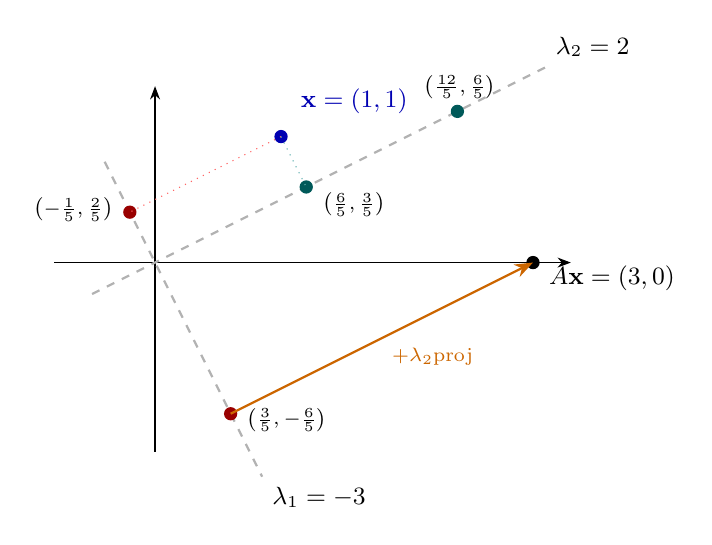
\begin{tikzpicture}[>=Stealth, scale=1.6]
  % Axes
  \draw[->] (-0.8,0)--(3.3,0) node[right]{\small};
  \draw[->] (0,-1.5)--(0,1.4) node[above]{\small};
  % Eigenspace lines (dashed)
  % lambda_1=-3: direction [1,-2], line y = -2x in range
  \draw[gray!60, dashed, thick] (-0.4,0.8)--(0.85,-1.7)
    node[below right, black]{\small $\lambda_1=-3$};
  % lambda_2=2: direction [2,1], line y=x/2 in range
  \draw[gray!60, dashed, thick] (-0.5,-0.25)--(3.1,1.55)
    node[above right, black]{\small $\lambda_2=2$};
  % Point x=(1,1)
  \fill[blue!70!black] (1,1) circle (1.5pt);
  \node[blue!70!black] at (1.08,1.1) [above right]{\small $\mathbf{x}=(1,1)$};
  % Projection onto lambda_1 eigenspace: (-1/5, 2/5)
  \fill[red!60!black] (-0.2,0.4) circle (1.5pt);
  \node at (-0.25,0.42)[left]{\scriptsize $\!\left(-\tfrac{1}{5},\tfrac{2}{5}\right)$};
  \draw[dotted, red!60] (1,1)--(-0.2,0.4);
  % Scaled projection lambda_1: (3/5, -6/5)
  \fill[red!60!black] (0.6,-1.2) circle (1.5pt);
  \node at (0.65,-1.25)[right]{\scriptsize $\left(\tfrac{3}{5},-\tfrac{6}{5}\right)$};
  % Projection onto lambda_2 eigenspace: (6/5, 3/5)
  \fill[teal!70!black] (1.2,0.6) circle (1.5pt);
  \node at (1.25,0.63)[below right]{\scriptsize $\left(\tfrac{6}{5},\tfrac{3}{5}\right)$};
  \draw[dotted, teal!60] (1,1)--(1.2,0.6);
  % Scaled projection lambda_2: (12/5, 6/5)
  \fill[teal!70!black] (2.4,1.2) circle (1.5pt);
  \node at (2.42,1.22)[above]{\scriptsize $\left(\tfrac{12}{5},\tfrac{6}{5}\right)$};
  % Ax = (3,0)
  \fill[black] (3,0) circle (1.5pt);
  \node at (3.05,0.05)[below right]{\small $A\mathbf{x}=(3,0)$};
  % Arrow indicating sum
  \draw[->,thick,orange!80!black] (0.6,-1.2)--(3,0)
    node[midway, below right]{\scriptsize $+\lambda_2\text{proj}$};
\end{tikzpicture}
\caption{Spectral decomposition: $A\mathbf{x}$ as the sum of scaled eigenspace projections
(red: $\lambda_1=-3$ contribution; teal: $\lambda_2=2$ contribution).}
\label{fig:721}
\end{figure}

\redheading{The Nondiagonalizable Case}

If $A$ is an $n\times n$ matrix that is not orthogonally diagonalizable, it may still
be possible to achieve considerable simplification in $P^T AP$ by choosing $P$ appropriately.
The following two theorems, stated without proof, illustrate this.

\begin{tcolorbox}[colback=red!4, colframe=red!60!black,
  title={\textbf{Theorem 7.2.3 --- Schur's Theorem}}, boxrule=0.5mm, arc=3mm]
If $A$ is an $n\times n$ matrix with real entries and real eigenvalues, then there is an
orthogonal matrix $P$ such that $P^T AP$ is an upper triangular matrix of the form
\begin{equation}
  P^T AP = \begin{bmatrix}
    \lambda_1 & \times & \times & \cdots & \times\\
    0 & \lambda_2 & \times & \cdots & \times\\
    0 & 0 & \lambda_3 & \cdots & \times\\
    \vdots & \vdots & \vdots & \ddots & \vdots\\
    0 & 0 & 0 & \cdots & \lambda_n
  \end{bmatrix}
  \tag{11}
\end{equation}
where $\lambda_1,\lambda_2,\ldots,\lambda_n$ are the eigenvalues of $A$ repeated according
to multiplicity. The factorization $A = PSP^T$ (where $S$ denotes the upper triangular matrix)
is called a \textbf{Schur decomposition} of $A$.
\end{tcolorbox}

\begin{tcolorbox}[colback=red!4, colframe=red!60!black,
  title={\textbf{Theorem 7.2.4 --- Hessenberg's Theorem}}, boxrule=0.5mm, arc=3mm]
If $A$ is an $n\times n$ matrix with real entries, then there is an orthogonal matrix $P$
such that $P^T AP$ is a matrix of the form
\begin{equation}
  P^T AP = \begin{bmatrix}
    \times & \times & \cdots & \times & \times & \times\\
    \times & \times & \cdots & \times & \times & \times\\
    0 & \times & \ddots & \times & \times & \times\\
    \vdots & \vdots & \ddots & \vdots & \vdots & \vdots\\
    0 & 0 & \cdots & \times & \times & \times\\
    0 & 0 & \cdots & 0 & \times & \times
  \end{bmatrix}
  \tag{13}
\end{equation}
in which every entry below the \emph{first subdiagonal} is zero. Such a matrix is said to
be in \textbf{upper Hessenberg form}. The factorization $A = PHP^T$ (where $H$ denotes
the upper Hessenberg matrix) is called an \textbf{upper Hessenberg decomposition} of $A$.
\end{tcolorbox}

\textit{Remark.} Unlike the diagonal entries in the Schur form~(11), the diagonal entries
in the Hessenberg form~(13) are usually \emph{not} the eigenvalues of $A$. In many
numerical algorithms the matrix is first converted to upper Hessenberg form to reduce
computation in subsequent steps.

\vspace{3mm}
\noindent\rule{\linewidth}{0.5pt}

\section*{Exercise Set 7.2}

\noindent\textit{In Exercises 1--6, find the characteristic equation of the given
symmetric matrix, then determine by inspection the dimensions of the eigenspaces.}

\begin{enumerate}

\item $\begin{bmatrix}1&2\\2&4\end{bmatrix}$

\item[3.] $\begin{bmatrix}1&1&1\\1&1&1\\1&1&1\end{bmatrix}$

\item[4.] $\begin{bmatrix}4&2&2\\2&4&2\\2&2&4\end{bmatrix}$

\noindent\textit{In Exercises 7--14, find a matrix $P$ that orthogonally diagonalizes $A$,
and determine $P^{-1}AP$.}

\item[7.] $A = \begin{bmatrix}6&2\sqrt{3}\\2\sqrt{3}&7\end{bmatrix}$

\item[9.] $A = \begin{bmatrix}-2&0&-36\\0&-3&0\\-36&0&-23\end{bmatrix}$

\item[11.] $A = \begin{bmatrix}2&-1&-1\\-1&2&-1\\-1&-1&2\end{bmatrix}$

\item[12.] $A = \begin{bmatrix}1&1&0\\1&1&0\\0&0&0\end{bmatrix}$

\noindent\textit{In Exercises 15--18, find the spectral decomposition of the matrix.}

\item[15.] $\begin{bmatrix}3&1\\1&3\end{bmatrix}$

\item[17.] $\begin{bmatrix}-3&1&2\\1&-3&2\\2&2&0\end{bmatrix}$

\noindent\textit{In Exercises 19--20, determine whether there exists a $3\times 3$
symmetric matrix whose eigenvalues are $\lambda_1=-1$, $\lambda_2=3$, $\lambda_3=7$ and
for which the corresponding eigenvectors are as stated. Find the matrix if it exists; if
not, explain why.}

\item[19.] $\mathbf{x}_1=\begin{bmatrix}0\\1\\-1\end{bmatrix}$,\quad
$\mathbf{x}_2=\begin{bmatrix}1\\0\\0\end{bmatrix}$,\quad
$\mathbf{x}_3=\begin{bmatrix}0\\1\\1\end{bmatrix}$

\item[21.] Let $A$ be a diagonalizable matrix with the property that eigenvectors
corresponding to distinct eigenvalues are orthogonal. Must $A$ be symmetric? Explain.

\item[22.] Assuming $b\neq 0$, find a matrix $A$ that orthogonally diagonalizes
$\begin{bmatrix}a&b\\b&a\end{bmatrix}$.

\noindent\textit{In Exercise 23, let $T_A\colon\mathbb{R}^2\to\mathbb{R}^2$ be
multiplication by $A$. Find two orthogonal unit vectors $\mathbf{u}_1$ and $\mathbf{u}_2$
such that $T_A(\mathbf{u}_1)$ and $T_A(\mathbf{u}_2)$ are orthogonal.}

\item[23.] \textbf{a.}\ $A=\begin{bmatrix}-1&1\\1&1\end{bmatrix}$
\hspace{20pt}
\textbf{b.}\ $A=\begin{bmatrix}1&2\\2&1\end{bmatrix}$

\noindent\textit{\textbf{Working with Proofs}}

\item[25.] Prove that if $A$ is any $m\times n$ matrix, then $A^T A$ has an orthonormal
set of $n$ eigenvectors.

\item[28.]
\textbf{a.}\ If $\mathbf{v}$ is any $n\times 1$ matrix and $I$ is the $n\times n$
identity matrix, prove that $I - \mathbf{v}\mathbf{v}^T$ is orthogonally diagonalizable.

\textbf{b.}\ Find a matrix $P$ that orthogonally diagonalizes $I - \mathbf{v}\mathbf{v}^T$ if
\[
  \mathbf{v} = \begin{bmatrix}1\\0\\1\end{bmatrix}
\]

\item[29.] Prove that if $A$ is a symmetric orthogonal matrix, then $1$ and $-1$ are
the only possible eigenvalues.

\end{enumerate}

\end{document}
